% !TEX root = ../notes_template.tex

\section*{5장 - 연습문제 풀이}

\subsection*{연습문제 \ref{ex-5-1}}

\begin{itemize}
\item[(1)] $(x,y)\in \mathbb R^2\setminus\{(0,0)\}$에 대하여
\begin{align*}
\dfrac{\partial u}{\partial x} &= \dfrac1{x^2+y^2} \cdot 2x = \dfrac{2x}{x^2+y^2} \\
\dfrac{\partial^2 u}{\partial x^2} &= \dfrac2{x^2+y^2} - \dfrac{2x}{(x^2+y^2)^2} \cdot (2x) 
= \dfrac{2y^2+2x^2-4x^2}{(x^2+y^2)^2} = \dfrac{2(y^2-x^2)}{(x^2+y^2)^2}.
\end{align*}
$x$, $y$에 대한 대칭식임을 이용하면
\[
\dfrac{\partial u}{\partial y}  = \dfrac{2y}{x^2+y^2}, \quad
\dfrac{\partial^2 u}{\partial y^2} = \dfrac{2(x^2-y^2)}{(x^2+y^2)^2}.
\]
따라서,
\[
\dfrac{\partial^2 u}{\partial x^2} + \dfrac{\partial^2 u}{\partial y^2}
= \dfrac{2(y^2-x^2)}{(x^2+y^2)^2} + \dfrac{2(x^2-y^2)}{(x^2+y^2)^2} = 0.
\]
$\mathbb R^2\setminus\{(0,0)\}$에서
$u\in C^2$이고 $\Delta u=0$이므로, $u$는 조화함수이다.
\item[(2)] 
$(x,y) \in \mathbb R^2$에 대하여
\begin{align*}
\dfrac{\partial u}{\partial x} &= e^x\sin y, \ \dfrac{\partial^2 u}{\partial x^2} = e^x\sin y, \\
\dfrac{\partial u}{\partial y} &= e^x\cos y, \ \dfrac{\partial^2 u}{\partial y^2} = e^x(-\sin y).
\end{align*}
따라서, 
$\dfrac{\partial^2 u}{\partial x^2} + \dfrac{\partial^2 u}{\partial y^2}
= e^x\sin y + e^x(-\sin y) = 0$.
$\mathbb R^2$에서
$u\in C^2$이고 $\Delta u=0$이므로, $u$는 조화함수이다.
\end{itemize}

\subsection*{연습문제 \ref{ex-5-2}}

$U$에 정의된 실변수 함수의 점별 연산에 대한 공간 $V$를 생각하자.
$V$는 벡터공간이 됨을 알고 있다.
$\Har(U)$가 점별 연산에 대하여 $V$의 부분공간을 이룬다는 것을 증명하자.
\begin{itemize}
\item[(S1)]
$U$의 모든 점에서 $0$을 대응시키는 상수함수 $\bs 0$가 $\Har(U)$에 속한다.
\[
\dfrac{\partial^2 \bs 0}{\partial x^2} + \dfrac{\partial^2 \bs 0}{\partial y^2} = 0+0=0.
\]
\item[(S2)] $u,v\in \Har(U)$라고 하면,
\begin{align*}
\dfrac{\partial^2 (u+v)}{\partial x^2} + \dfrac{\partial^2 (u+v)}{\partial y^2}
&= \dfrac{\partial^2 u}{\partial x^2} + \dfrac{\partial^2 v}{\partial x^2}
+ \dfrac{\partial^2 u}{\partial y^2}+ \dfrac{\partial^2 v}{\partial y^2} \\ 
&= \left(\dfrac{\partial^2 u}{\partial x^2} + \dfrac{\partial^2 u}{\partial y^2} \right)
+ \left( \dfrac{\partial^2 v}{\partial x^2} + \dfrac{\partial^2 v}{\partial y^2} \right) \\
&= 0+0=0.
\end{align*}
\item[(S3)] $\alpha\in\mathbb R$이고, $u\in\Har(U)$이면,
\begin{align*}
\dfrac{\partial^2 (\alpha\cdot u)}{\partial x^2} + \dfrac{\partial^2 (\alpha\cdot u)}{\partial y^2}
&= \alpha\cdot \dfrac{\partial^2 u}{\partial x^2} 
+ \alpha \cdot \dfrac{\partial^2 u}{\partial y^2} \\
&= \alpha \left( \dfrac{\partial^2 u}{\partial x^2} + \dfrac{\partial^2 u}{\partial y^2} \right)
= \alpha\cdot 0 = 0.
\end{align*}
이상에서 $\Har(U)$는 점별 연산에 대하여 실 벡터공간이 된다.
\end{itemize}

\subsection*{연습문제 \ref{ex-5-3}}

$u:=x=\Re(z)$, $\tilde u:= x+y = \Re(z-iz)$는 모두 $\mathbb R^2$의
조화함수이다.
두 함수의 점별 곱은 $u\cdot \tilde u = x\cdot(x+y) = x^2 +xy$이다.
\[
\dfrac{\partial^2 (u\cdot \tilde u)}{\partial x^2} 
+ \dfrac{\partial^2 (u\cdot \tilde u)}{\partial y^2}
= \dfrac{\partial}{\partial x}(2x+y) + \dfrac{\partial}{\partial y}(x) = 2 + 0 = 2\ne 0.
\]
따라서 두 조화함수의 점별 곱이 반드시 조화함수가 되는 것은 아니다.

\subsection*{연습문제 \ref{ex-5-4}}

\begin{itemize}
\item[(1)] $u=e^x\sin y$라고 하자. $u+iv$가 복소해석함수인 $v$를 찾으면 된다.
코시-리만 방정식을 만족해야 하므로
\[
\dfrac{\partial v}{\partial x} = - \dfrac{\partial u}{\partial y}= -e^x\cos y.
\]
$y$를 고정하고 $x$로 적분하면 $v=-e^x \cos y + C(y)$를 얻는다. 
여기서 $C(y)$는 $y$에만 의존하는 적분상수이다.
\[
\dfrac{\partial v}{\partial  y} = e^x\sin y + C'(y) 
= \dfrac{\partial u}{\partial x} = e^x \sin y
\]
이므로 $C'(y)=0$에서 $C(y)=K$이다.
$v:= -e^x \cos y$로 두자. 그러면
\begin{align*}
u+iv &= e^x\sin y + i(-e^x\cos y) = e^x (\sin y - i\cos y) \\
&= -ie^x(\cos y +i\sin y) = -i \exp(x+iy) = -i\exp(z),
\end{align*}
여기서 $z=x+iy$이고
$u+iv = -i\exp z$는 실제로 복소해석함수이다.
따라서 $v:=-e^x\cos y$는 $u:=e^x\sin y$의 조화결레함수이다.

\item[(2)] $u= x^3_2xy^2-2y$라고 하자. $u+iv$가 복소해석함수인 $v$를 찾으면 된다.
코시-리만 방정식을 만족해야 하므로
\[
\dfrac{\partial v}{\partial x} = - \dfrac{\partial u}{\partial y}= 6xy+2.
\]
$y$를 고정하고 $x$로 적분하면 
\[
v = 6\dfrac{x^2}{2}y + 2x + C(y) = 3x^2y +2x+ C(y).
\]
여기서 $C(y)$는 $y$에만 의존하는 적분상수이다.
\[
\dfrac{\partial v}{\partial  y} = 3x^2 + C'(y) 
= \dfrac{\partial u}{\partial x} = 3x^2 - 3y^2
\]
이므로 $C'(y)=-3y^2$에서 
\[
 C(y) = -3\dfrac{y^3}{3} + C  = -y^3+C.
\]
$v:= 3x^2y+2x-y^3$으로 두자. 그러면
\begin{align*}
u+iv &= x^3-3xy^2 -2y +i(3x^2y + 2x-y^3) \\  
&= x^3 +3x(iy)^2 + 3x^2(iy) +(iy)^3 -2y +i2x \\
&= (x+iy)^3 + 2i(x+iy) = z^3+2iz.
\end{align*}
여기서 $z=x+iy$이고
$u+iv =z^3+2iz$는 실제로 복소해석함수이다.
따라서 $v:=3x^2y+2x-y^3$는 $u:=x^3_2xy^2-2y$의 조화결레함수이다.

\item[(3)] $u= x(1+2y)$라고 하자. $u+iv$가 복소해석함수인 $v$를 찾으면 된다.
코시-리만 방정식을 만족해야 하므로
\[
\dfrac{\partial v}{\partial x} = - \dfrac{\partial u}{\partial y}= -2x.
\]
$y$를 고정하고 $x$로 적분하면 
\[
v = 2\dfrac{x^2}{2} + C(y) = -x^2 + C(y).
\]
여기서 $C(y)$는 $y$에만 의존하는 적분상수이다.
\[
\dfrac{\partial v}{\partial  y} =  C'(y) 
= \dfrac{\partial u}{\partial x} = 1+2y
\]
이므로
\[
 C(y) = y + 2\cdot \dfrac{y^2}2 + C = y + y^2 + C.
\]
$v:= -x^2+y+y^2$으로 두자. 그러면
\begin{align*}
u+iv &= x(1+2y) + i(-x^2+y+y^2) = x+iy + 2xy + i(y^2-x^2) \\
&= x + iy -i( (x^2-y^ 2) +i2xy ) = x+ iy -i(x+iy)^2 \\
&=  z- iz^2.
\end{align*}
여기서 $z=x+iy$이고
$u+iv =z-iz^2$는 실제로 복소해석함수이다.
따라서 $v:=-x^2 + y+y^2$는 $u:=x(1+2y)$의 조화결레함수이다.

\end{itemize}

\subsection*{연습문제 \ref{ex-5-5}}

$v$를 $u$의 조화켤레함수라고 하자.
그러면 $f:= u+iv$는 $\mathbb C\setminus \{0\}$에서
복소해석함수이다. 
따라서 $h:= z^2 \exp(-f(z))$가 $\mathbb C\setminus \{0\}$에서
복소해석함수이다. 
\begin{align*}
|h| & = |z|^2|\exp(-f(z))| = |z|^2 e^{-\Re(f(z))} = |z|^2e^{-u}
= |z|^2e^{-\log |z|^2} \\
&= |z|^2\cdot \dfrac1{|z|^2} = 1.
\end{align*}
이로부터 $h$가 $\mathbb C\setminus \{0\}$에 포함된 모든 원판에서 상수함수가 되어야 한다.
따라서 $h'=0$이다.
한편,
\[
h' = 2z \exp(-f(z)) + z^2\exp(-f(z))\cdot (-f'(z))
\]
에서
\[
f'(z) = \dfrac2z
\]
이고 $1/z$가 $\mathbb C\setminus \{0\}$에서 부정적분을 갖게 된다.
이제 경로 $\gamma(t) =\exp(it)$, $0\le t \le 2\pi$를 따라 적분하면,
\[
2\cdot 2\pi i = \int_\gamma \dfrac2z dz = \int_\gamma f'(z)dz = 0
\]
가 되어 모순이 생긴다.

따라서 $u$는 $\mathbb C\setminus \{0\}$에서 조화켤레함수를 가질 수 없다.

\subsection*{연습문제 \ref{ex-5-6}}

$u:=x^3+y^3$이라 하자.
$f$가 복소해석함수라면, $u$는 조화함수이다.
그런데, $x\ne y$에 대하여
\[
\dfrac{\partial^2 u}{\partial x^2} + \dfrac{\partial^2 u}{\partial y^2}
= \dfrac{\partial}{\partial x}(3x^2) + \dfrac{\partial}{\partial y}(3y^2)
= 6x + y6 = 6(x+y) \ne 0.
\]
따라서 $f=u+iv$가 복소해석함수가 되는 $v$를 찾을 수 없다.

\subsection*{연습문제 \ref{ex-5-7}}

$u$가 조화함수일 때, $\dfrac{\partial u}{\partial x}$, $\dfrac{\partial u}{\partial y}$도
조화함수가 됨을 보이면 충분하다.
$u$가 무한번 미분가능함을 알고 있으므로,
\begin{align*}
\dfrac{\partial^2}{\partial x^2}\left(\dfrac{\partial u}{\partial x}\right) 
+ \dfrac{\partial^2}{\partial y^2}\left(\dfrac{\partial u}{\partial x}\right) 
&= \dfrac{\partial}{\partial x}\left(\dfrac{\partial^2 u}{\partial x^2}\right) 
+ \dfrac{\partial}{\partial y}\left(\dfrac{\partial^2 u}{\partial y\partial x}\right)  \\
&= \dfrac{\partial}{\partial x}\left(-\dfrac{\partial^2 u}{\partial y^2}\right) 
+ \dfrac{\partial}{\partial y}\left(\dfrac{\partial^2 u}{\partial x\partial y}\right)  \\
&= \dfrac{\partial}{\partial x}\left(-\dfrac{\partial^2 u}{\partial y^2}\right) 
+ \dfrac{\partial}{\partial x}\left(\dfrac{\partial}{\partial y}
\left(\dfrac{\partial}{\partial y}u \right)\right)  \\
&= \dfrac{\partial}{\partial x}\left(-\dfrac{\partial^2 u}{\partial y^2}
+\dfrac{\partial^2 u}{\partial y^2} \right) 
= \dfrac{\partial}{\partial x}(0) = 0.
\end{align*}
같은 방법으로
\begin{align*}
\dfrac{\partial^2}{\partial x^2}\left(\dfrac{\partial u}{\partial y}\right) 
+ \dfrac{\partial^2}{\partial y^2}\left(\dfrac{\partial u}{\partial y}\right)  
&= \dfrac{\partial}{\partial y}\left(\dfrac{\partial^2 u}{\partial x^2}\right) 
+ \dfrac{\partial}{\partial y}\left(\dfrac{\partial^2 u}{\partial y^2}\right)  \\
&= \dfrac{\partial}{\partial y} \left(
\dfrac{\partial^2 u}{\partial x^2} + \dfrac{\partial^2 u}{\partial y^2} \right)
= \dfrac\partial{\partial y}(0) = 0.
\end{align*}

\subsection*{연습문제 \ref{ex-5-8}}

\begin{itemize}
\item[(1)]  $b(x) = p(x) = c_0 + c_1 x + \cdots + c_d x^d$이라 하면,
\[
p(z) := p(x+iy) = c_0 + c_1 z + \cdots + c_d z^d
\]
은 전해석함수이다. 따라서 $h:= \Re(p(x+iy))$는 조화함수이다.
또한, 모든 $x\in\mathbb R$에 대하여
\[
h(x,0) = \Re(p(x+i0)) =\Re(p(x)) = \Re(b(x)) = b(x)
\]
를 만족한다.

\item[(2)]  $b(z):= b(x+iy) = \dfrac1{1+z^2}$은 $z=i$에서 정의되지 않는다.
하지만,
\[
\dfrac{i}{z+i}
\]
는 상반평면에서 복소해석함수이고, 따라서 실수부가 조화함수이다.
또한, 모든 $x\in\mathbb R$에 대하여
\[
h(x,0) = \dfrac{0+1}{x^2+(0+1)^2} = \dfrac1{x^2+1} = b(x)
\]
를 만족한다.
\end{itemize}

\subsection*{연습문제 \ref{ex-5-9}}

$f$가 전해석함수이고 실수부가 $u$라고 하자.
($\mathbb C$는 단순연결영역임을 상기하자.)
그러면, $\exp(-f)$도 전해석함수이다.
모든 $x,y \in\mathbb R$에 대하여 $u(x,y) >0$이므로,
\[
|\exp(-f)| = e^{-\Re(f)} = e^{-u} \le 1.
\]
리우비유 정이에 의해, $\exp(-f)$는 상수함수이다.
따라서 $|\exp(-f)|$도 상수이고, $e^{-u}$도 상수함수이다.
결론적으로, 실수 로그값 $\log(e^{-u}) = -u$도 상수이므로
$u$는 상수함수가 된다.

\subsection*{연습문제 \ref{ex-5-10}}

\begin{itemize}
\item[(1)] $z=r\exp(i\theta)$에 대하여
\[
\exp\left(-\dfrac1{z^4}\right) = \exp\left( -\dfrac1{r^4} \exp(-i4\theta)\right)
\]
이므로, $r= 1/n$, $4\theta = -\pi$로 택하면, 즉,
\[
z_n := \dfrac1n \exp\left( -i\dfrac\pi4 \right) =: x_n + iy_n.
\]
$u(x_n,y_n) = \exp(-n^4\exp(i\pi)) = \exp(-n^4(-1)) = e^{n^4}$이다.
그러면, $(x_n, y_n)\to (0,0)$이지만, $u(x_n, y_n) \to 0$은 아니므로,
$u$는 $(0,0)$에서 연속이 아니다.

\item[(2)] 

\begin{align*}
u(x,0) &= \exp\left( - \dfrac1{(x+0i)^4} \right) = e^{-1/x^4}, \\
u(0,y) &= \exp\left( - \dfrac1{(0+yi)^4} \right) = \exp\left( - \dfrac1{i^4y^4}\right)
= \exp\left( - \dfrac1{1\cdot y^4} \right) = e^{-1/y^4}.
\end{align*}

\item[(3)] 
\[
\dfrac{\partial u}{\partial x}(0,0) =
\lim_{x\to 0} \dfrac{u(x,0) - u(0,0)}{x-0} = \lim_{x\to 0} \dfrac{e^{-1/x^4}-0}x
= \lim_{x\to 0} \dfrac{e^{-1/x^4}}x = 0.
\]
여기서 마지막 등식은 다음과 사실로부터 얻는다.
\[
e^{1/x^4} = 1 + \dfrac1{x^4} + \dfrac1{2!}\left(\dfrac1{x^4}\right)^2 
+ \cdots > \dfrac1{x^4}
\]
이므로 $0\le \left| \dfrac{e^{-1/x^4}}x\right| \le |x|^3$.

유사한 방법으로 $\dfrac{\partial u}{\partial x}(0,0) =0$을 보일 수 있다.
따라서,
\begin{align*}
\dfrac{\partial^2 u}{\partial x^2} (0,0)
&= \lim_{x\to0} \dfrac{ \dfrac{\partial u}{\partial x}(x,0) -\dfrac{\partial u}{\partial x}(0,0)}
{x-0} = \lim_{x\to0} \dfrac{\dfrac d{dx}e^{-1/x^4} - 0}x \\
&= \lim_{x\to0}  \dfrac{e^{-1/x^4}\cdot \dfrac{-4}{x^5}}x
= \lim_{x\to0} \dfrac{-4e^{-1/x^4}}{x^6} = 0.
\end{align*}
이를 위해, 부등식
$e^{1/x^4} = 1 + \dfrac1{x^4} + \dfrac1{2!}\left(\dfrac1{x^4}\right)^2 + \cdots
> \dfrac1{2x^8}$로부터 
$0\le \left| \dfrac{e^{-1/x^4}}{x^6}\right| \le 2|x|^2$이 성림함을 이용하였다.

유사한 방법으로,
\[
\dfrac{\partial^2u}{\partial y^2}(0,0)=0
\]
을 보일 수 있고, 결론적으로 
$\dfrac{\partial^2 u}{\partial x^2}(0,0) + \dfrac{\partial^2 u}{\partial y^2}(0,0) = 0+0=0$.
\end{itemize}

\subsection*{연습문제 \ref{ex-5-11}}
\begin{itemize}
\item[(1)] 
$z_0\in D_1$이라 하자. 그러면, $\varphi(z_0)\in D_2$이다.
중심을 $\varphi(z_0)$로 하고 충분히 작은 반지름 $\epsilon>0$을 갖는
원판 $\Delta$가 $\Delta \subset D_2$와 $\varphi^{-1}(\Delta) \subset D_1$를
만족하도록 잡을 수 있다.
$\Delta$가 단순연결영역이므로, $\Delta$에서 $g=\Re(G)$를 만족하는
복소해석함수 $G$가 존재한다.
복소해석함수 $\varphi|_{\varphi^{-1}(\Delta)}: \varphi^{-1}(\Delta)\to \Delta$와
$G: \Delta \to \mathbb C$의 합성함수는 복소해석함수이고,
$\Re(G\circ\varphi|_{\varphi^{-1}(\Delta)})$는 $\varphi^{-1}(\Delta)$에서
조화함수이다. 
한편, $z\in \varphi^{-1}(\Delta)$에 대하여, 
$\varphi|_{\varphi^{-1}(\Delta)}(z)  = \varphi(z)\in \Delta$이고
\[
(G\circ \varphi|_{\varphi^{-1}(\Delta)})(z)
= G(\varphi(z)) = g(\varphi(z)) = (g\circ \varphi)(z).
\]
따라서, $(g\circ \varphi|_{\varphi^{-1}(\Delta)}$은 
$\varphi^{-1}(\Delta)$에서 조화함수이다.
특히, $z_0\in \varphi^{-1}(\Delta)$에서 
$\Delta(g\circ \varphi)(z_0)=0$이다.
$z_0\in D_1$의 선택을 임의로 할 수 있으므로, $g\circ \varphi$는 $D_1$에서 조화함수이다.

\item[(2)] $h:D_2\to\mathbb R$이 조화함수이면, 앞의 증명에서
$h\circ \varphi : D_1 \to \mathbb R$도 조화함수이다.

이제 $h\circ \varphi : D_1 \to \mathbb R$가 조화함수라고 가정하자.
그러면, 앞의 증명에서 $(h\circ\varphi)\circ\varphi^{-1}:D_2 \to \mathbb R$도 조화함수이다.
항등함수 $z\mapsto z (z\in D_2)$를 ${\rm id}_{D_2}: D_2 \to D_2$로 쓰면,
$(h\circ \varphi)\circ \varphi^{-1} = h\circ(\varphi \circ \varphi^{-1})
= h\circ ({\rm id}_{D_2}) =h$이므로,
$h:D_2\to\mathbb R$도 조화함수이다. 

\item[(3)] \

\begin{figure}[h!]
\begin{center}
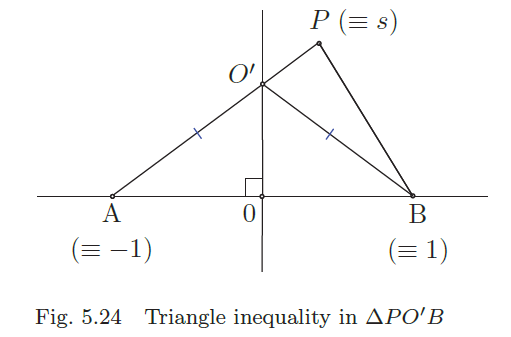
\includegraphics[width=0.5\textwidth]{./Solution/figs/fig-5-24}
\end{center}
\caption{$\Delta PO'B$에 대한 삼각부등식
}
\label{fig-5-24}
\end{figure}

그림 \ref{fig-5-24}의 $\Delta PO'B$에서 삼각부등식을 쓰면,
$\mathbb H$의 점 $s(\equiv P)$에 대하여
\begin{align*}
|s+1| = \ell(PA) = \ell(PO') + \ell(O'A)
&= \ell(PO') + \ell (O'B) \\
&> \ell(PB) = |s-1|.
\end{align*}
여기서, $O'$이 선분  $AB$의 수직이등분선임을 이용하여
세번째 등식을 얻었다.
따라서 모든 $s\in\mathbb H$에 대하여 $\varphi(s)\in \mathbb D$를 얻는다.
함수 $\varphi$가 복소해석함수임은 분명하므로, $s\in\mathbb H$에  대하여
\[
\varphi'(s) = 1\cdot \dfrac1{s+1} + (s-1)\cdot
\left( - \dfrac1{(s+1)^2} \right) = \dfrac{s+1-s+1}{(s+1)^2}
= \dfrac2{(s+1)^2}.
\]
이제 함수  $\psi: \mathbb D \to \mathbb H$를
\[
\psi(s) = \dfrac{1+z}{1-z}, \quad z\in\mathbb D
\]
로 정의하자.
($\psi$는
방정식 $z= \varphi(s) = \dfrac{s-1}{s+1}$을 $s$에 대하여 푸는 방법으로
$\varphi^{-1}$를 구한 것이다.)

\begin{figure}[h!]
\begin{center}
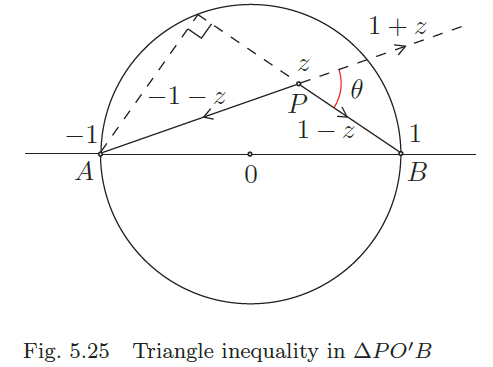
\includegraphics[width=0.5\textwidth]{./Solution/figs/fig-5-25}
\end{center}
\caption{원주각을 이용한 $\angle APB$
}
\label{fig-5-25}
\end{figure}

그림 \ref{fig-5-25}에서 원 위의 임의의 점에 대하여
지름 $AB$에 대한 원주각이 $90^\circ$이므로,
$\mathbb D$의 점 $P(\equiv z)$에 대하여
$\angle APB >90^\circ$이다. 따라서,
\[
\Re(\psi(z)) = \Re\left( \dfrac{1+z}{1-z} \right)
= |\psi(z)| \cos\theta = |\psi(z)| \cos(\pi - \angle APB) >0.
\]
따라서 모든 $z\in \mathbb D$에 대하여 $\psi(z)\in \mathbb H$이다.
함수 $\psi$는 $\mathbb D$에서 복소해석함수이고, $z\in\mathbb D$에 대하여
\[
\psi'(z) = 1\cdot \dfrac1{1-z} + (1+z)\cdot \left(\dfrac1{(1-z)^2}\right)
= \dfrac{1-z+1+z}{(1-z)^2} = \dfrac2{(1-z)^2}.
\]
끝으로, 모든 $s\in\mathbb H$에 대하여
\[
(\psi\circ \varphi)(s) = \dfrac{1+\dfrac{s-1}{s+1}}{1-\dfrac{s-1}{s+1}}
= \dfrac{s+1+s-1}{s+1-s+1} = \dfrac{2s}2 = s
\]
이고, 모든 $z\in\mathbb D$에 대하여 
\[
(\varphi\circ\psi)(z) = \dfrac{\dfrac{1+z}{1-z}-1}{\dfrac{1+z}{1-z}+1}
= \dfrac{1+z-1+z}{1+z+1-z} = \dfrac{2z}2 = z.
\]
따라서 $\varphi$는 전단사함수이고 $\varphi^{-1}=\psi$이다.


\end{itemize}
